% !TEX root = Dokumentation_SysSpec.tex
Das folgende Kontextdiagramm soll eine Übersicht geben in welchem Rahmen sich das zu
realisierende System bewegt. Auf der Abbildung sind die Umsysteme sowie der Informations-
Austausch definiert.

\begin{figure}[H]
	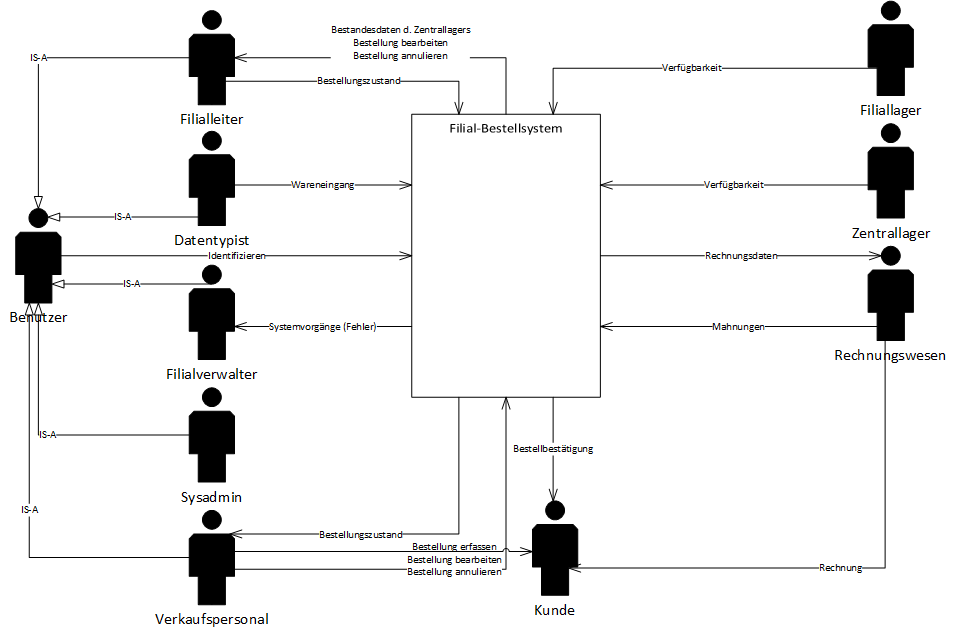
\includegraphics[width=1.0\linewidth]{Images/kontextdiagram}
	\caption{Kontextdiagram}
	\label{fig:kontextdiagram}
\end{figure}

Das Rechnungswesen und Zentrallager sind externe Systeme mit definierten oder noch zu definierenden Schnittstellen.

Die Umsysteme und Akteure sind wie folgt definiert:\\
\textbf{Umsysteme}:
\begin{itemize}
\item Zentrallager: Nachbestellungen des lokalen Filiallagers werden an das Zentrallager gesendet.
\item Rechnungswesen: Das Rechnungswesen wird für Bestell-Bestätigungen, Rechnungsversand und Mahnungsprüfungen verwendet.
\item Filiallager: Lagerung der in der Filiale verkauften Artikel. Filiallager und Applikation müssen jederzeit einen übereinstimmenden Datenbestand haben.
\end{itemize}

\textbf{Akteuere}:
\begin{itemize}
\item Benutzer: Bestehend aus Filialverwalter, Filialleiter, Verkaufspersonal und Datentypist, bezeichnet alle Nutzer der Applikation. Die einzelnen Aktionen sind in der Use Case Übersicht ersichtlich
\item Sysadmin: Gemäss Anforderungen kein eigentlicher Benutzer. Für konfigurative Anpassungen könnte ein Zugriff notwendig sein
\item Kunde: Interaktion mit der Applikation wird via Verkaufspersonal abgewickelt.
\end{itemize}